\documentclass[12pt,a4paper]{article}
\usepackage{amsmath,amscd,amsbsy,amssymb,latexsym,url,bm,amsthm}
\usepackage{epsfig,graphicx,subfigure}
\usepackage{enumitem,balance}
\usepackage{wrapfig}
\usepackage{mathrsfs,euscript}
\usepackage[usenames]{xcolor}
\usepackage{hyperref}
\usepackage{mathrsfs}
\usepackage[vlined,ruled,linesnumbered]{algorithm2e}
\hypersetup{colorlinks=true,linkcolor=black}

\newtheorem{theorem}{Theorem}
\newtheorem{lemma}[theorem]{Lemma}
\newtheorem{proposition}[theorem]{Proposition}
\newtheorem{corollary}[theorem]{Corollary}
\newtheorem{exercise}{Exercise}
\newtheorem*{solution}{Solution}
\newtheorem{definition}{Definition}
\theoremstyle{definition}

\renewcommand{\thefootnote}{\fnsymbol{footnote}}

\newcommand{\postscript}[2]
 {\setlength{\epsfxsize}{#2\hsize}
  \centerline{\epsfbox{#1}}}

\renewcommand{\baselinestretch}{1.0}

\setlength{\oddsidemargin}{-0.365in}
\setlength{\evensidemargin}{-0.365in}
\setlength{\topmargin}{-0.3in}
\setlength{\headheight}{0in}
\setlength{\headsep}{0in}
\setlength{\textheight}{10.1in}
\setlength{\textwidth}{7in}
\makeatletter \renewenvironment{proof}[1][Proof] {\par\pushQED{\qed}\normalfont\topsep6\p@\@plus6\p@\relax\trivlist\item[\hskip\labelsep\bfseries#1\@addpunct{.}]\ignorespaces}{\popQED\endtrivlist\@endpefalse} \makeatother
\makeatletter
\renewenvironment{solution}[1][Solution] {\par\pushQED{\qed}\normalfont\topsep6\p@\@plus6\p@\relax\trivlist\item[\hskip\labelsep\bfseries#1\@addpunct{.}]\ignorespaces}{\popQED\endtrivlist\@endpefalse} \makeatother

\begin{document}
\noindent

%========================================================================
\noindent\framebox[\linewidth]{\shortstack[c]{
\Large{\textbf{Lab02-Divide and Conquer}}\vspace{1mm}\\
CS214-Algorithm and Complexity, Xiaofeng Gao, Spring 2021.}}
\begin{center}
\footnotesize{\color{red}$*$ If there is any problem, please contact TA Haolin Zhou. }

\footnotesize{\color{blue}$*$ Name: Wendi Chen  \quad Student ID: 519021910071 \quad Email: chenwendi-andy@sjtu.edu.cn}
\end{center}

\begin{enumerate}
\item
    \textit{Recurrence examples.} Give asymptotic upper and lower bounds for $T(n)$ in each of the following recurrences. Assume that $T(n)$ is constant for sufficiently small $n$. Make your bounds as tight as possible.
\begin{enumerate}
	\item $T(n)=4 T(n / 3)+n \log n$
	\item $T(n)=4 T(n / 2)+n^{2} \sqrt{n}$
	\item $T(n)=T(n-1)+n$	
	\item $T(n)=2T(\lfloor \sqrt n\rfloor)+\log n$
\end{enumerate}
\begin{solution}
	~
	\begin{enumerate}
	    \item We try to find the upper and lower bounds by using the \textbf{master theorem} according to \emph{Introduction to Algorithm}. \\
	    In this case, we have $a = 4$, $b = 3$, $f(n) = n\log n$, and $n^{\log_{b}{a}} = n^{\log_{3}{4}} = \Omega(n^{1.2}) $. Since $f(n) = O(n^{\log_{b}{a}-\epsilon})$, where $\epsilon = 0.1$, we can apply case 1 of the master theorem and conclude that the solution is $T(n) = \Theta(n^{\log_{3}{4}})$. Thus, we find the asymptotic upper and lower bounds for $T(n)$ that $T(n) = \Omega(n^{\log_{3}{4}}) = O(n^{\log_{3}{4}})$.
	    
	    \item In this case, we have $a = 2$, $b = 4$, $f(n) = n^2\sqrt{n}$, and $n^{\log_{b}{a}} =n^{\log_{4}{2}}= n^{0.5}$. Since $f(n) = \Omega(n^{0.5+\epsilon})$, where $\epsilon = 2$, case 3 applies if we can show that the regularity condition holds for $f(n)$. For sufficiently large $n$, we have $af(\frac{n}{b}) = 2(\frac{n}{4})^{2.5} = \frac{1}{16}n^{2.5}= cf(n)$ for $c = \frac{1}{16}$. Consequently, by case 3, the solution to the recurrence if $T(n) = \Theta(n^{2} \sqrt{n})$, which means $T(n) = \Omega(n^{2} \sqrt{n}) = O(n^{2} \sqrt{n})$.
	    
	    \item Without loss of generality, we assume that $T(n) = 1$. Then we have $T(n) = T(n-1) + n = T(n-2) + n +(n-1) = n + (n-1) + \dots + 1 = \frac{n(n+1)}{2}  = \Theta(n^2)$. Thus, we have $T(n) = \Omega(n^2)= O(n^2)$.
	    \item We can do some algebraic manipulation. Without loss of generality, we can assume $\sqrt{n}$ to be integers. Let $m = \log n$, then we have
	    \begin{align*}
	        T(2^m) = 2T(2^{m/2})+m 
	    \end{align*}
	    Then,set $S(m) = T(2^m)$, we get
	    \begin{align*}
	        S(m)= 2S(m/2)+m 
	    \end{align*}
	    Here, we have $a = 2$, $b=2$, $f(n) = n$, and $f(m) = \Theta(m^{\log_{b}{a}}) = \Theta(m^{\log_{2}{2}}) = \Theta(m)$. By case 2, we get S(m) = $\Theta(m\log m)$. Then $T(n) =\Theta( \log n \log\log n)$. Thus $T(n) = \Omega( \log n \log\log n) = O( \log n \log\log n)$.
	\end{enumerate}
\end{solution}
\item
\textit{Divide-and-conquer.} Given an integer array $A[1..n]$ and two integers $lower \le upper$, design an algorithm using \textbf{divide-and-conquer} method to count the number of ranges $(i,j)$ ($1 \leq i \leq j \leq n$) satisfying
$$
    lower \leq \sum_{k=i}^{j}{A[k]} \leq upper.
$$
\textbf{Example:}

Given $A = [1,-1,2]$, $lower = 1$, $upper = 2$, return 4.

The resulting four ranges are $(1,1)$, $(3,3)$, $(2,3)$ and $(1,3)$.

\begin{enumerate}
\item
Complete the implementation in the provided C/C++ source code {\color{blue}(The source code \emph{Code-Range.cpp} is attached on the course webpage)}.
\item
Write a recurrence for the running time of the algorithm and solve it by recurrence tree {\color{blue}(You can modify the figure sources \emph{Fig-RecurrenceTree.vsdx} or \emph{Fig-RecurrenceTree.pptx} to illustrate your derivation)}.
\item
Can we use the Master Theorem to solve the recurrence above? Please explain your answer.
\end{enumerate}
\begin{solution}
~
\begin{enumerate}
    \item Please refer to \emph{Code-Range.cpp}.
    \item According to the code, we implement binary search to find $m$ and $n$, whose time complexity is $O(\log n)$. In each recursion, we execute \emph{merge\_count} for $\lfloor \frac{n}{2} \rfloor$ elements and  $\lceil \frac{n}{2} \rceil$ elements. And then execute \emph{binary\_search} for $\lceil \frac{n}{2} \rceil$ elements $\lfloor \frac{n}{2} \rfloor$ times. At last, we sort $n$ elements, whose time complexity is $O(n\log n)$. Assuming that when there are $n$ elements, the time complexity is $T(n)$, then the recurrence is
    \begin{align}
        T(n) = T(\lfloor \frac{n}{2} \rfloor) + T(\lceil \frac{n}{2} \rceil) + 2\lfloor \frac{n}{2} \rfloor O(\log\lceil \frac{n}{2} \rceil) + O(n\log n)
    \end{align}
    For convenience, we assume $n$ is power of 2 and $k = log n+1$. Then by the definition of $O$ notation, we have
    \begin{align}
        T(n) = 2T(\frac{n}{2}) + O(n\log n)
    \end{align}
    Thus, we get the recurrence tree.\\
    \begin{figure}[htbp]
    \centering
    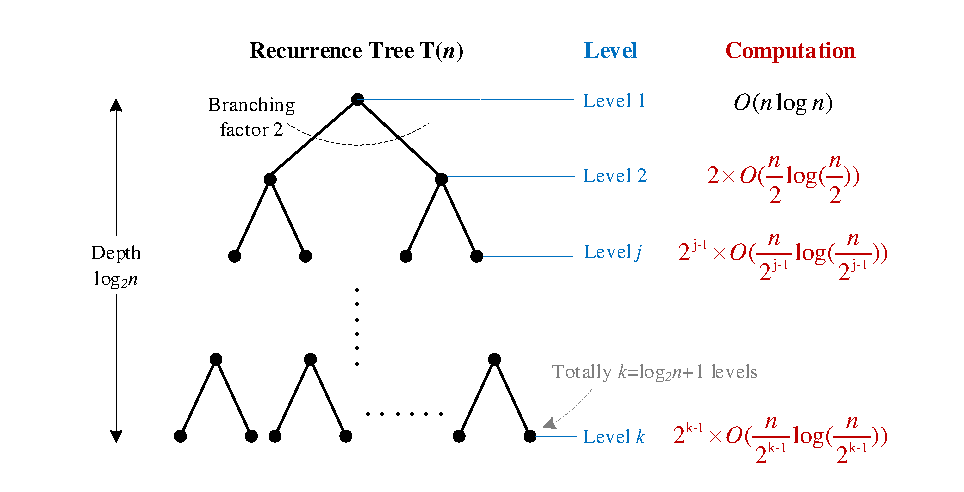
\includegraphics[width=0.78\textwidth]{Fig-RecurrenceTree.pdf}
    \caption{The Recurrence Tree of the Algorithm in \emph{Code-Range.cpp}.}\label{Fig-Transposition}
    \end{figure}
    ~\\
    According to the recurrence tree above, the total work done can be calculated by
    \begin{align}
        \begin{split}
            \sum_{j=1}^{\log n+1}(2^{j-1}\times O(\frac{n}{2^{j-1}}\log(\frac{n}{2^{j-1}}))) &= \sum_{j=1}^{\log n+1}O(n(\log n -(j-1)))\\
        &= O(n\log n(\log n+1)-n\frac{(\log n+1)(\log n +2)}{2})\\
        &= O(n(\log n)^2)
        \end{split}
    \end{align}
    \item Unfortunately, we can't solve the recurrence by the typical Master Theorem. However, we can generalize the theorem to solve this problem.\\
    According to the Master Theorem, we have $a = 2$, $b=2$, $f(n) = n\log n$, and $n^{log_{b}{a}} = n^{log_{2}{2}} = n$. Obviously, $n\log n = \Omega(n)$, but for any $\epsilon>0$, $f(n) = O(n^{1+\epsilon})$. So, for this recurrence, it falls into the gap between case 2 and case 3 of the Master Theorem. \\
    In fact, we can generalize the Master Theorem and have the conclusion that if $f(n) = \Theta(n^{\log_{b}a}(\log n)^k)$, then $T(n) = \Theta(n^{\log_{b}a}(\log n)^{k+1})$. This can be proved by recurrence tree. By this, we can solve the recurrence and get
    \begin{align}
        T(n) = \Theta(n(\log n)^2)
    \end{align}
\end{enumerate}
\end{solution}
\item
\textit{Transposition Sorting Network.} A comparison network is a \textbf{transposition network}  if each comparator connects adjacent lines, as in the network in Fig.~\ref{Fig-Transposition}.

\begin{figure}[htbp]
    \centering
    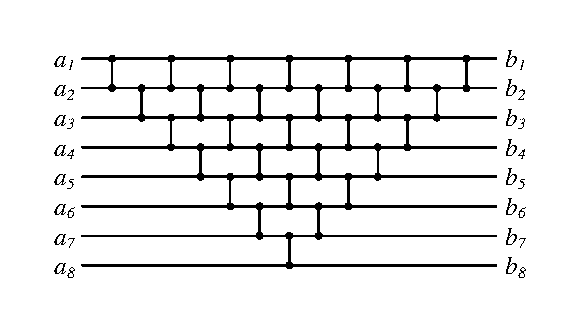
\includegraphics[width=0.4\textwidth]{Fig-Transposition.pdf}
    \caption{A Transposition Network Example}\label{Fig-Transposition}
\end{figure}

\begin{enumerate}
\item Prove that a transposition network with $n$ inputs is a sorting network if and only if it sorts the sequence $\langle n, n-1, \cdots, 1 \rangle$. {\color{blue}(Hint: Use an induction argument analogous to the \emph{Domain Conversion Lemma}.)}
\item {\color{red}{(Optional Sub-question with Bonus)}} Given any $n \in \mathbb{N}$, write a program using Tkinter in Python to draw a figure similar to Fig.~\ref{Fig-Transposition} with $n$ input wires.
\end{enumerate}
\begin{solution}
~
\begin{enumerate}
    \item \textbf{`Only if'} is easy to prove, because when a transposition network is a sorting network, it can definitely sort the sequence $\langle n, n-1, \cdots, 1 \rangle$.\\
    ~\\
    Then we'll prove \textbf{`if'}, which means if a transposition network sorts the sequence $\langle n, n-1, \cdots, 1 \rangle$, it is a sorting network. At the very beginning, we're wondering what information are provided by a totally revered sequence. Since a totally revered sequence has the greatest number of \textbf{reversed pair}, a natural idea is to consider the relation between the number of reversed pairs of it and that of a ordinary sequence. It's kind of complex, so we need to introduce some symbols and explanations.\\
    \begin{enumerate}
        \item Although a sorting network is a parallel sorting algorithm. We can also view it serially. In terms of the output depth of the comparators, we can denote them by $C_1,\dots,C_m$.
        \item We define $f(A,i,k)$ as the output of the $i$-th wire after the $k$-th comparator when the input sequence is $A$. $k=0$ implies the input elements.
        \item We define sequence $A = \langle n, n-1, \cdots, 1 \rangle$.
    \end{enumerate}
    Next, we'll prove if sometimes two elements on two wires are relatively orderly when the input is $A$, then the two elements on the positions are also relatively orderly when the input is any sequence of $1,2,\dots,n$. That is, when $i<j$
    \begin{equation}
        P(k):f(A,i,k)<f(A,j,k) \Rightarrow f(B,i,k)<f(B,j,k)
    \end{equation}
    \textbf{Basis.} When k = 0, there is no element pair satisfying $i<j$ and $f(A,i,k)<f(A,j,k)$. Thus, $P(0)$ is true.\\
    \textbf{Induction.} If $P(k)$ is true, we are trying to prove $P(k+1)$ is true. Assume the input wires of $C_k$ are the $i$-th wire and $i+1$-th wire. We can prove this by cases.
    \begin{enumerate}
        \item $p=i$, $q = i+1$ and $f(A,p,k+1)<f(A,q,k+1)$. By the definition of a comparator, we have $f(B,p,k+1)<f(B,q,k+1)$.
        \item $p<i$, $q = i$ and $f(A,p,k+1)<f(A,q,k+1)$. In this case, we have $f(B,p,k+1)=f(B,p,k)$. Beside, we have
        \begin{align}
        \begin{split}
            f(A,p,k) &= f(A,p,k+1)\\
            &<f(A,q,k+1)\\
            &\leq min(f(A,i,k),f(A,i+1,k))
        \end{split}
        \end{align}
        Thus, we get
        \begin{align}
        \begin{split}
            f(B,p,k+1)&=f(B,p,k)\\
            &<min(f(B,i,k),f(B,i+1,k))\\ 
            &= f(B,i,k+1)\\ 
            &= f(B,q,k+1)
        \end{split}
        \end{align}
        \item $p<i$, $q = i+1$ and $f(A,p,k+1)<f(A,q,k+1)$. In this case, we also have $f(B,p,k+1) = f(B,p,k)$. Beside, we have
        \begin{align}
        \begin{split}
            f(A,p,k) &= f(A,p,k+1)\\
            &<f(A,q,k+1)\\
            &\leq min(f(A,i,k),f(A,i+1,k))\\
            &\leq max(f(A,i,k),f(A,i+1,k))
        \end{split}
        \end{align}
        If $max(f(A,i,k),f(A,i+1,k)) = f(A,i+1,k)$, we can derive $f(B,p,k)<f(B,i+1,k)$ and $f(B,i,k)<f(B,i+1,k)$, then we get
         \begin{align}
        \begin{split}
            f(B,p,k+1)&=f(B,p,k)\\
            &<f(B,i+1,k)\\ 
            &= max(f(B,i,k),f(B,i+1,k))\\ 
            &= f(B,i+1,k+1)\\
            &= f(B,q,k+1)
        \end{split}
        \end{align}
        \item $p\neq i$, $p\neq i+1$, $q\neq i$, $q \neq  i+1$ and $f(A,p,k+1)<f(A,q,k+1)$. Then we get $f(A,p,k)=f(A,p,k+1)<f(A,q,k+1)=f(A,q,k)$, which implies $f(B,p,k+1)=f(B,p,k)<f(B,q,k)=f(B,q,k+1)$.
        \item $p=i+1$, $q > i+1$ and $f(A,p,k+1)<f(A,q,k+1)$. We can prove this like ii.
        \item $p=i$, $q > i+1$ and $f(A,p,k+1)<f(A,q,k+1)$. We can prove this like iii.
    \end{enumerate}
    ~\\
    The cases above implies $P(K+1)$ is true. By mathematical induction, $P(m)$ is true. Since the network sorts $A$, $f(A,i,m)<f(A,j,m)$ are true for all $i<j$. Thus, $f(B,i,m)<f(B,j,m)$ are true for all $i<j$, which implies the network sorts $B$. Then this network is a sorting network.
    % \begin{enumerate}
    %     \item We define $\mathscr{C}$ as a collection  of swaps $f_i$. A \textbf{swap} means that if the larger one of two adjacent elements is placed before the smaller one, then change the order of the two.
    %     \begin{align*}
    %         \mathscr{C} = \{f_1,\dots,f_{t}\}
    %     \end{align*}
    %     \item When we apply a swap $f_i \in \mathscr{C}$ to a sequence $\mathbf{a}$, it's denoted by $f_i(\mathbf{a})$. We can also apply several swaps to $\mathbf{a}$, like $f_{i_s}\circ\dots\circ f_{i_1}(\mathbf{a})$.
    %     \item If $a_i>a_j$ while $i<j$, then we call $(a_i,a_j)$ a \textbf{reversed pair}. 
    %     \item We define the $k$-depth output of a transposition network when the maximum depth of wires is $k$.
    %     \item \textbf{Lemma 1.} Every swap or comparator in the transposition network will at most reduce the number of the reversed pair in one sequence by one.
    %     \item \textbf{Lemma 2.} For any sequence $\mathbf{a}$ of $1,2,\dots,n$, there exist a composition of $f_i \in \mathscr{C}$ satisfying $f_{i_s}\circ\dots\circ f_{i_1}(\langle n, n-1, \cdots, 1 \rangle) = \mathbf{a}$. 
    % \end{enumerate}
    % Lemma 1 is obvious, because the two elements it swaps are adjacent and this operation will not affect their relative position to other elements. Lemma 2 can be proved through a reversed process of bubble sort. If we want to bubble sort sequence $\mathbf{a}$ non-decreasingly, what we do is to swap the adjacent elements and put the larger one before the smaller one, which is actually the opposite of $f_i$. Thus, we can just reverse the process of bubble sort and find $f_{i_s}\circ\dots\circ f_{i_1}$, which implies lemma 2 is true.\\
    % ~\\
    % Next, we'll try to prove that if the transposition network transforms $\langle n, n-1, \cdots, 1 \rangle$ into sequence $\mathbf{b}$(with $k$ reversed pairs), then for any sequence $f_{i_s}\circ\dots\circ f_{i_1}(\langle n, n-1, \cdots, 1 \rangle)$, the number of reversed pairs in the output sequence is no more than $k$.\\
    % ~\\
    % \textbf{Basis.} The $0$-depth output is the input sequence $\langle n, n-1, \cdots, 1 \rangle$ (with $\frac{n(n-1)}{2}$ reversed pairs, which is the most of all possible sequences). For $f_{i_s}\circ\dots\circ f_{i_1}(\langle n, n-1, \cdots, 1 \rangle)$, the number of reversed pairs can't exceed $\frac{n(n-1)}{2}$.

    \item Please refer to \emph{Code-TranspositionSortingNetwork.py}.
    
    \begin{figure}[htbp]
    \centering
    \subfigure[$n=4$]{
    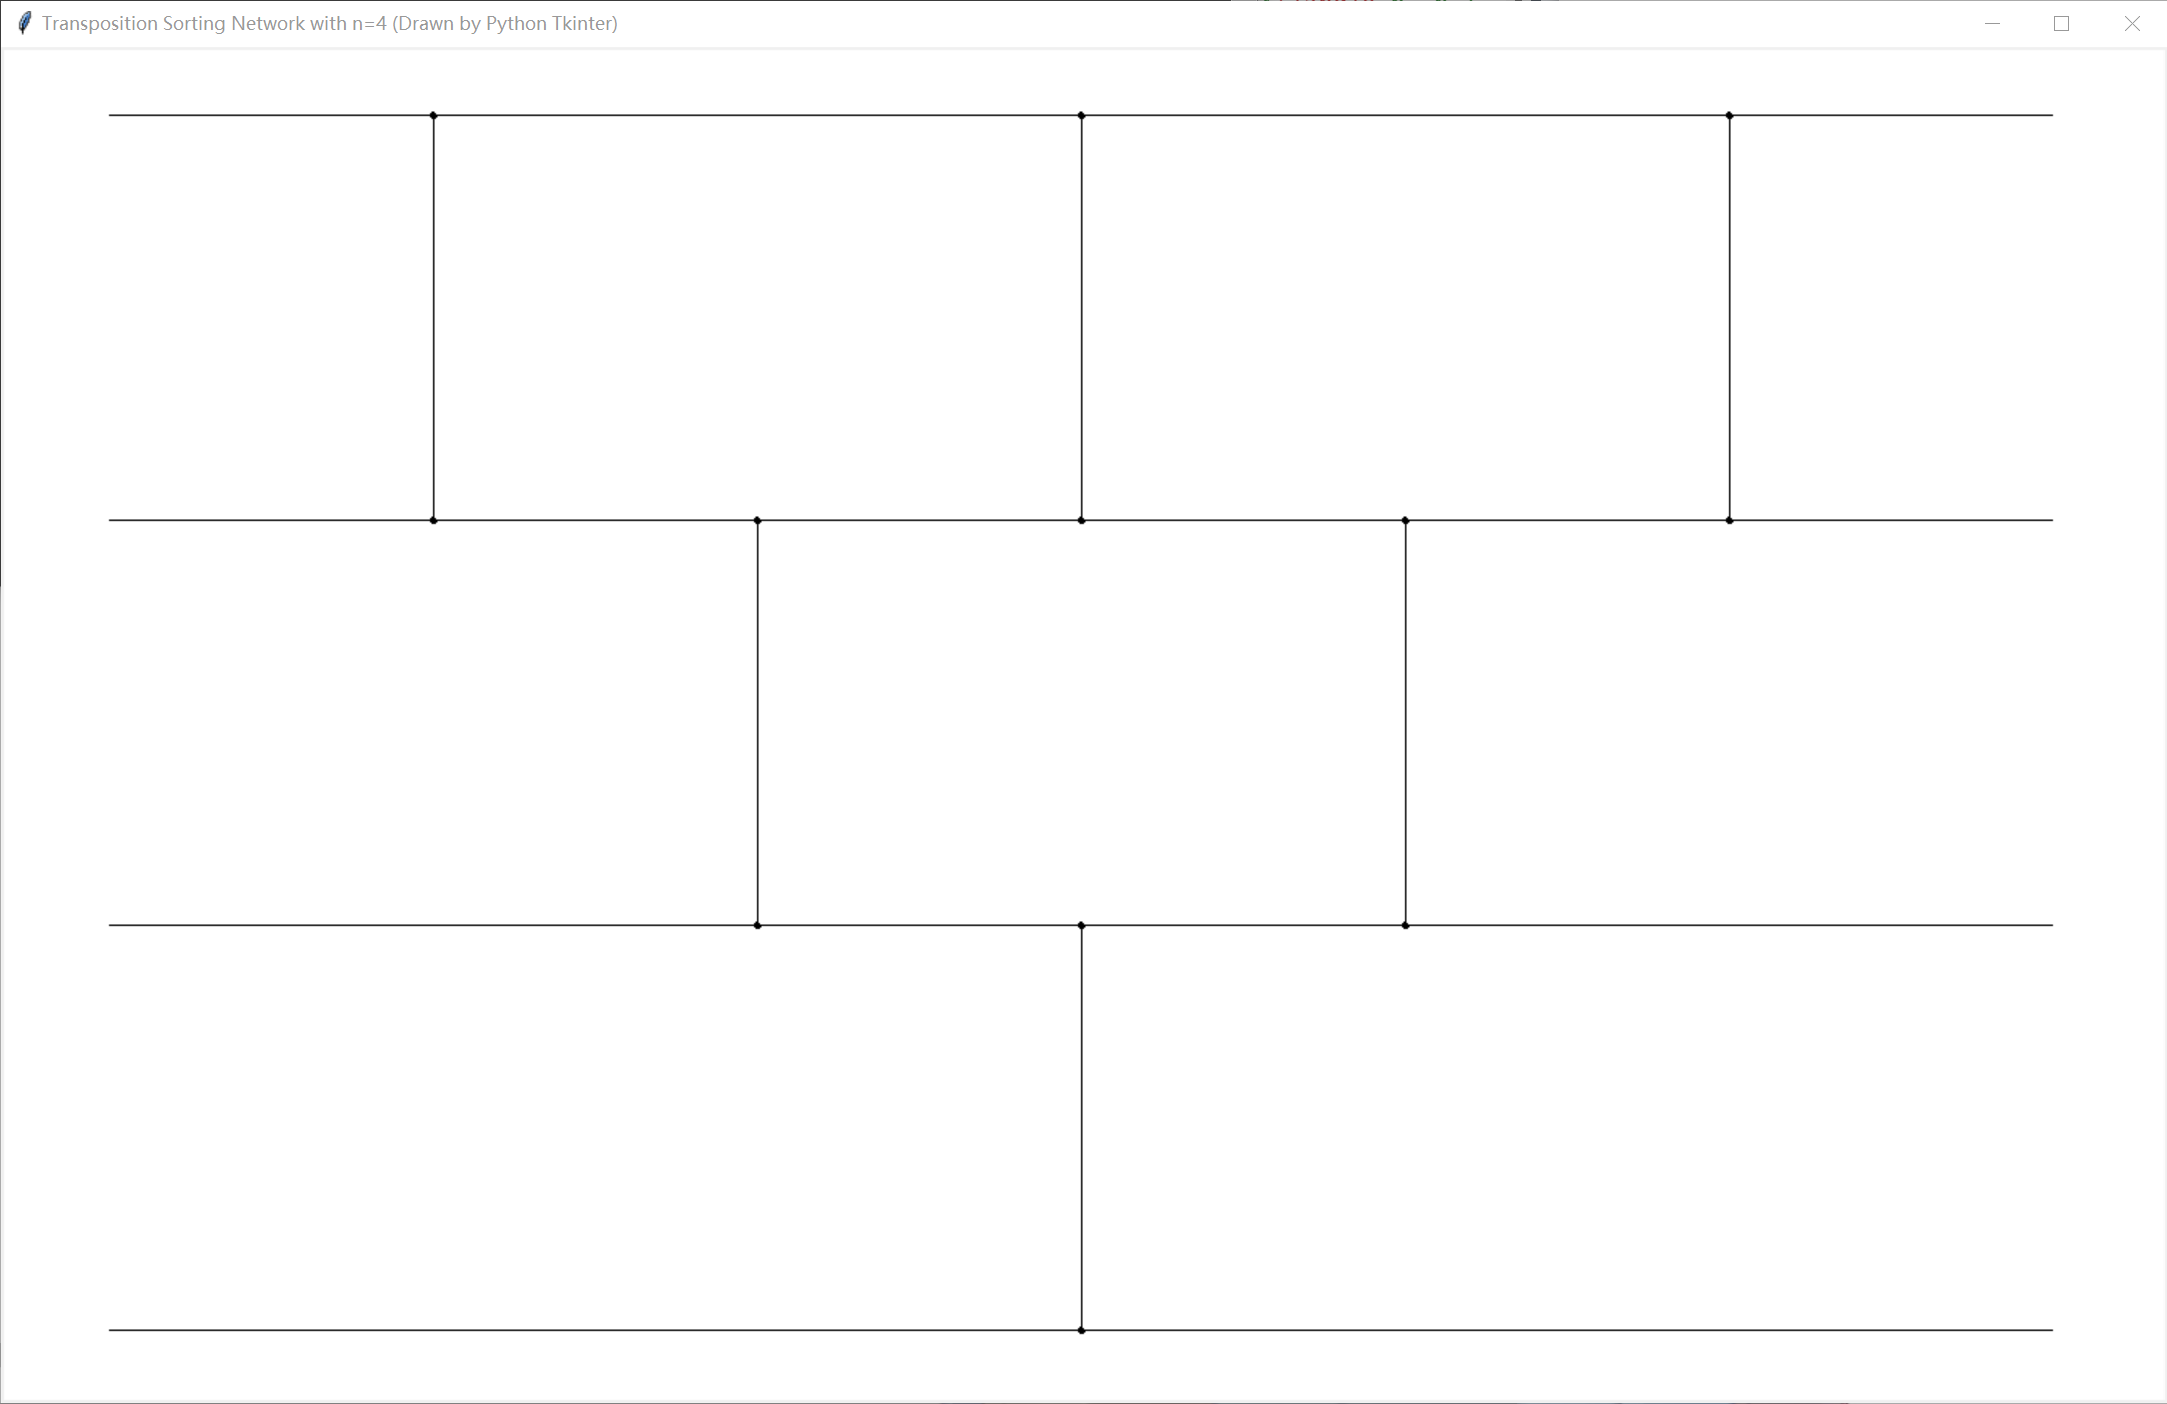
\includegraphics[width=7.5cm]{Fig-Trans4.png}
    %\caption{fig1}
    }
    \quad
    \subfigure[$n=16$]{
    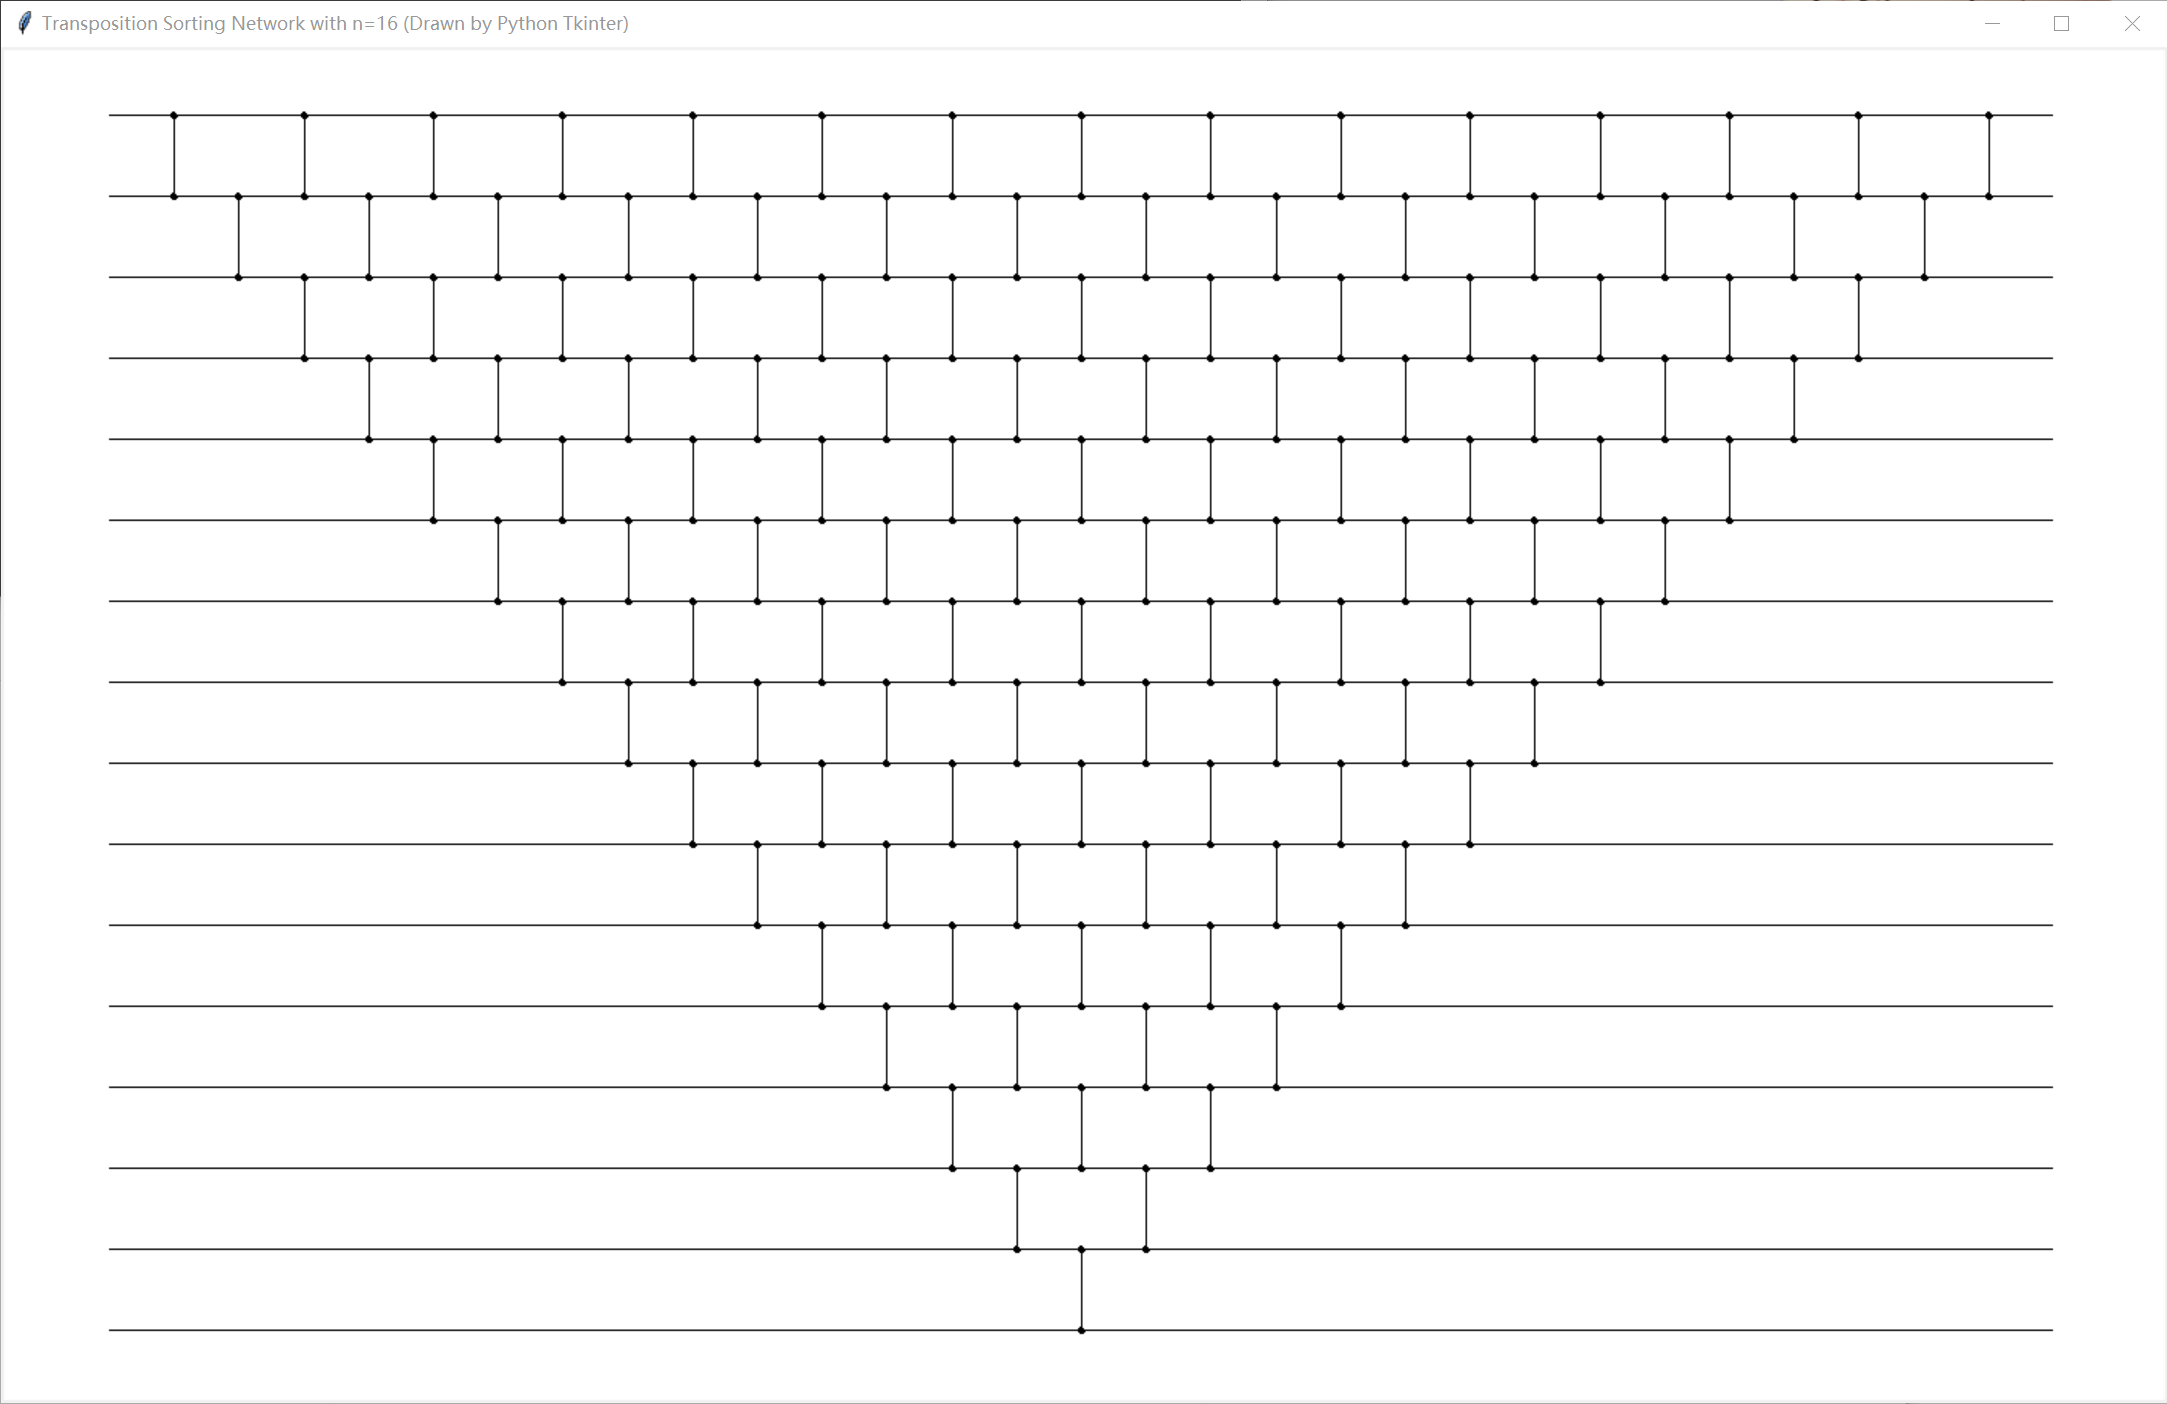
\includegraphics[width=7.5cm]{Fig-Trans16.png}
    }
    \quad
    \subfigure[$n=32$]{
    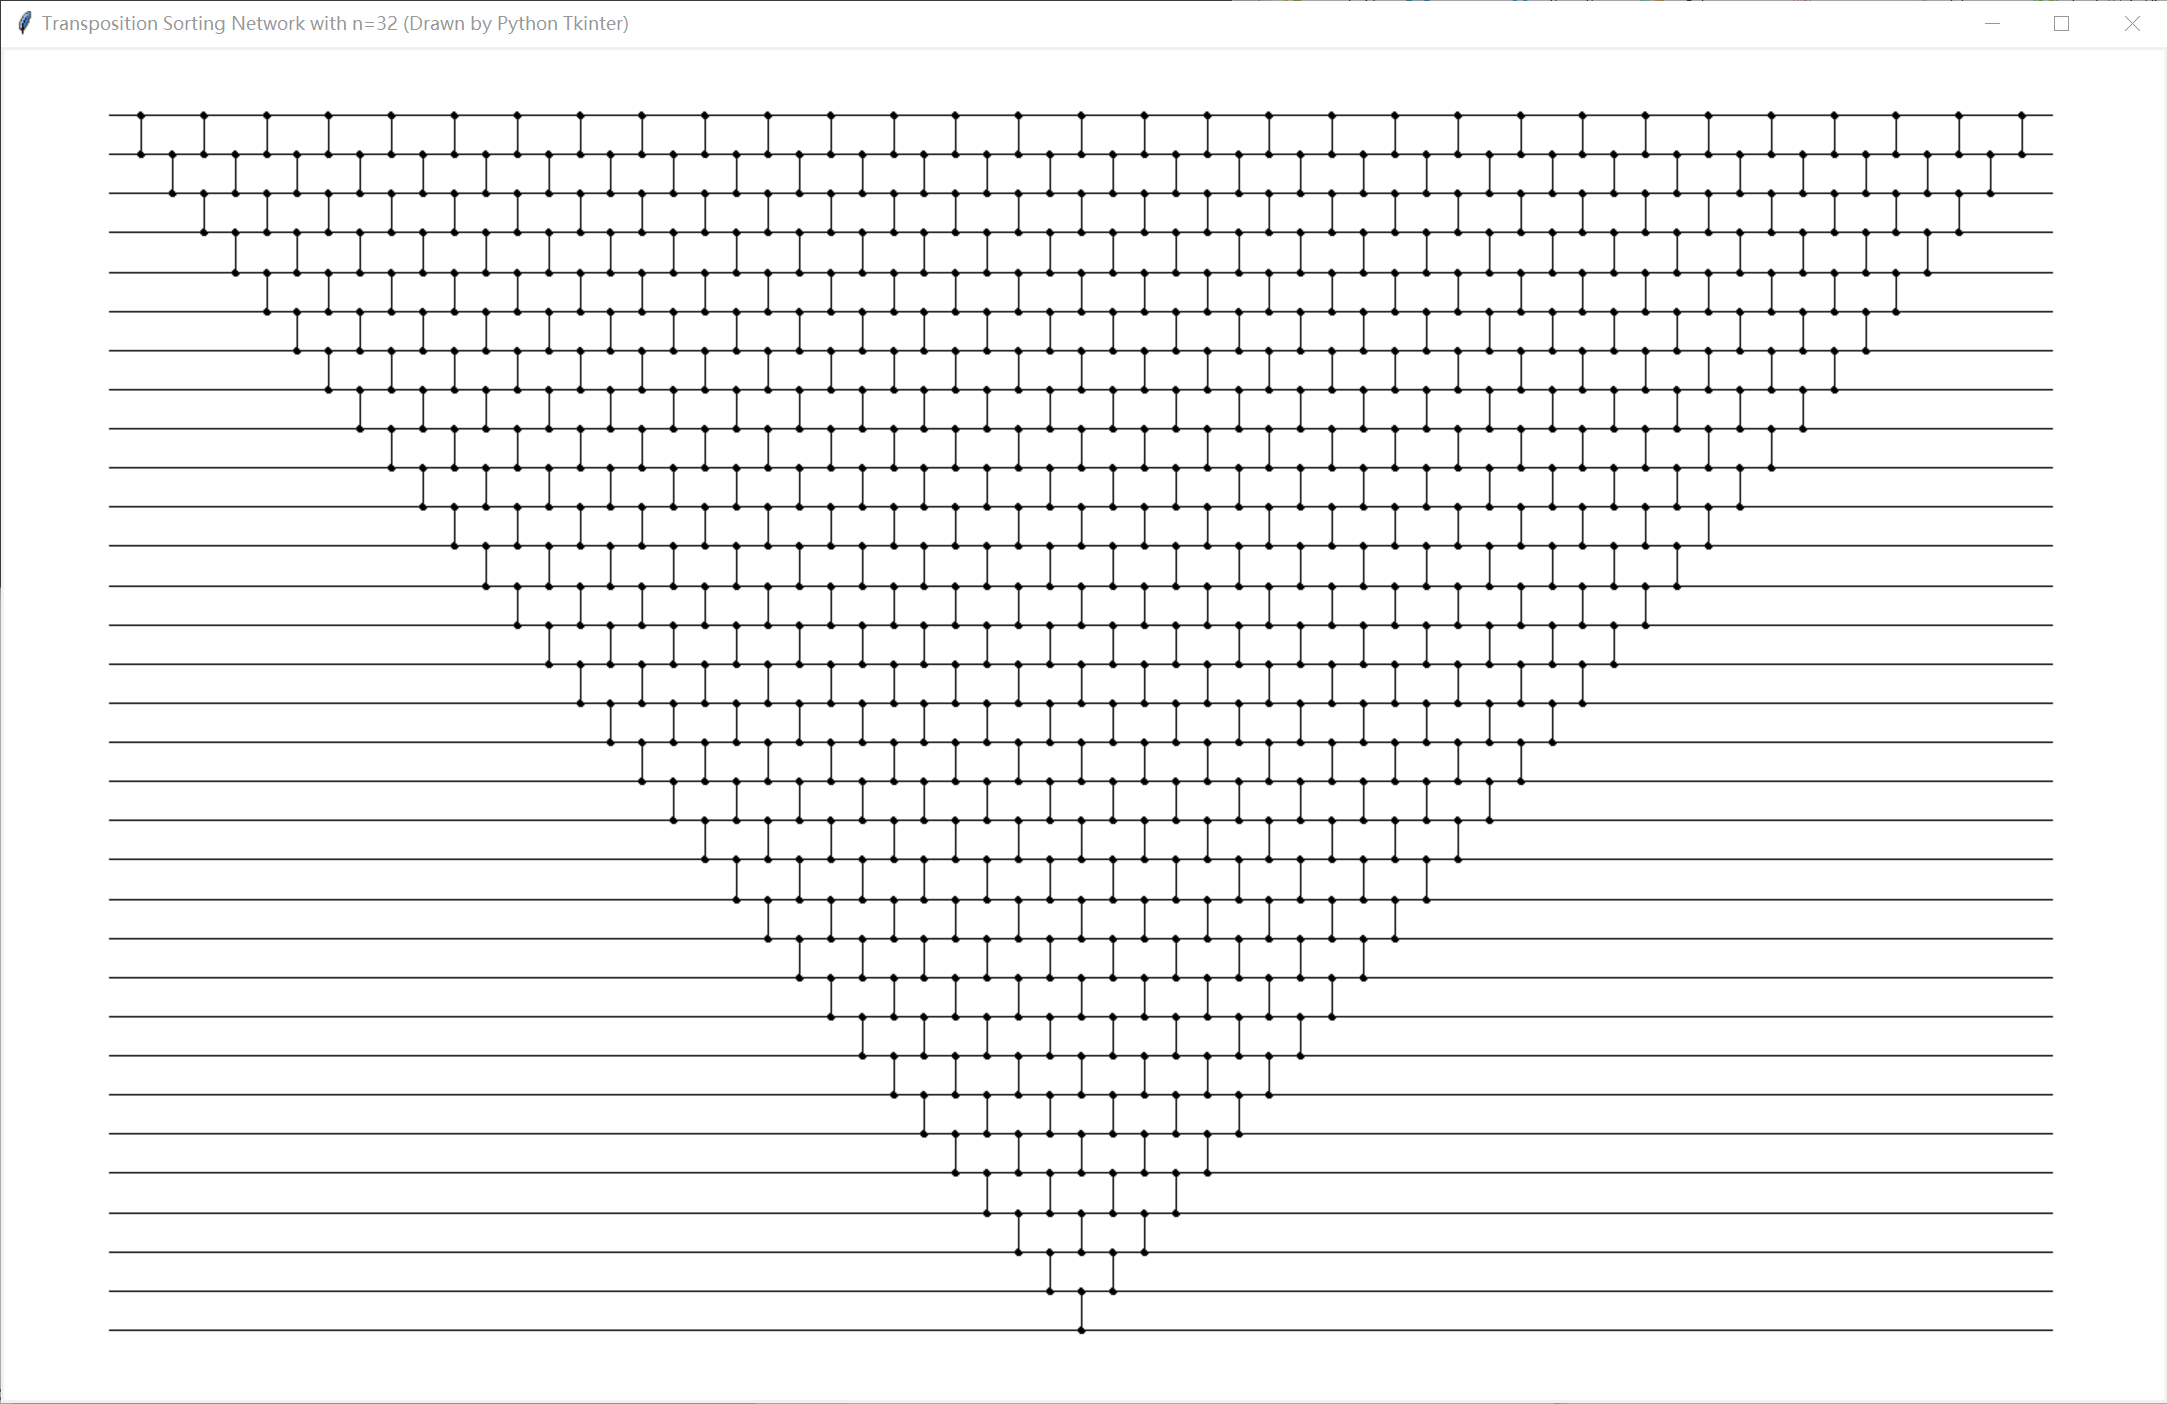
\includegraphics[width=7.5cm]{Fig-Trans32.png}
    }
    \quad
    \subfigure[$n=64$]{
    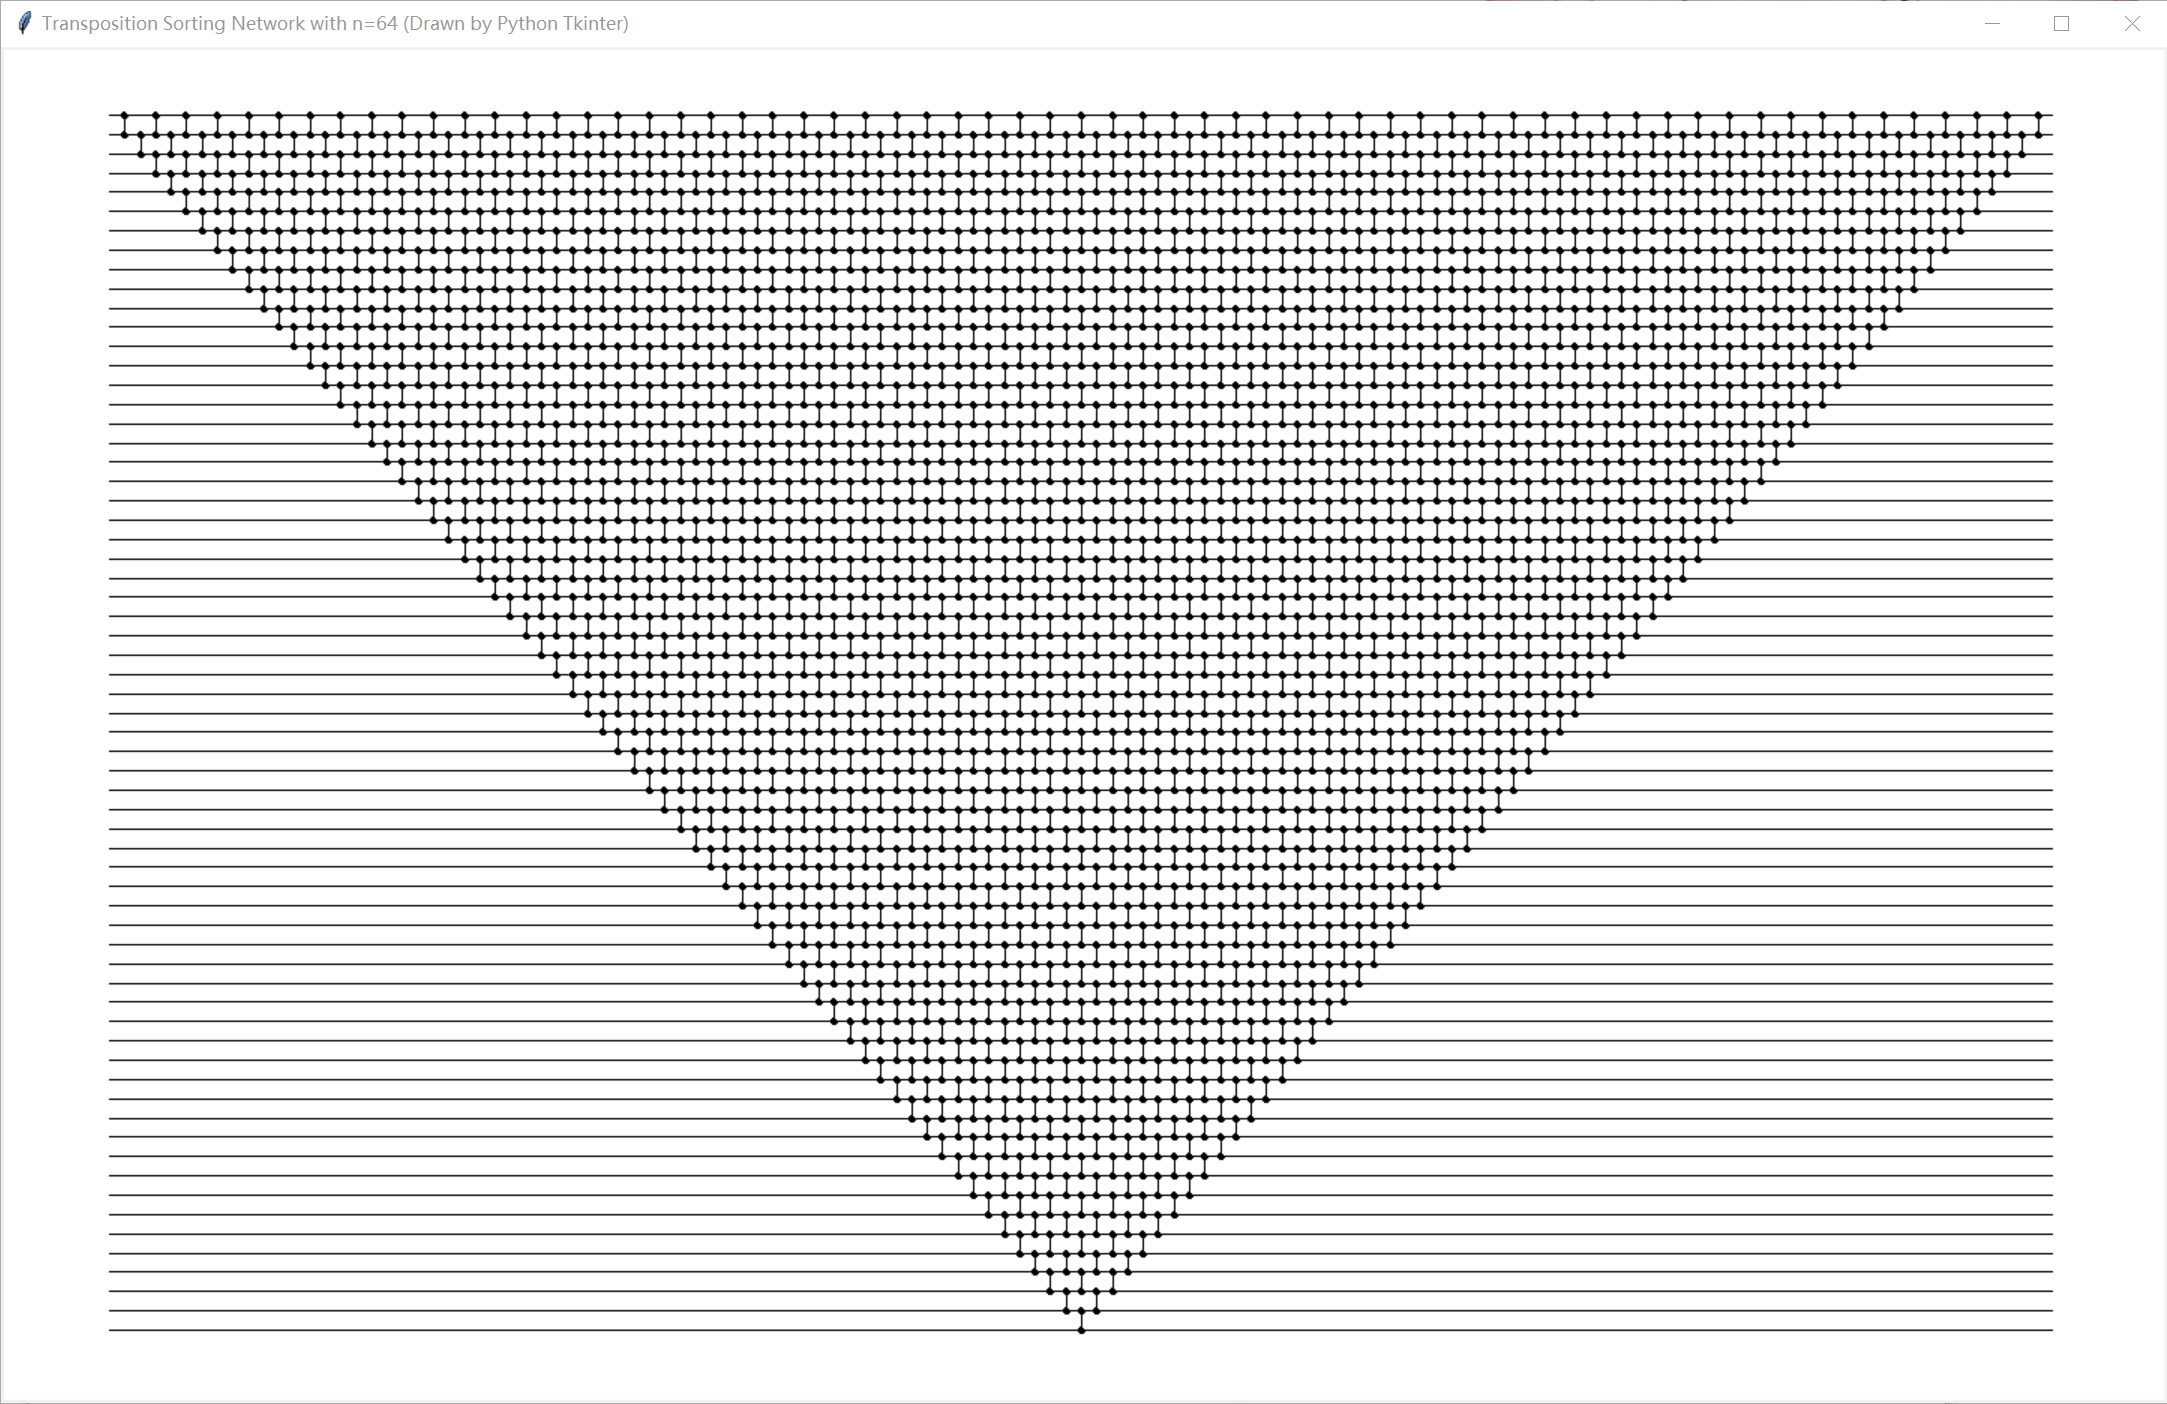
\includegraphics[width=7.5cm]{Fig-Trans64.png}
    }
    \caption{ Transposition Networks Generated with Tkinter}
    \end{figure}
\end{enumerate}
\end{solution}
\end{enumerate}

%========================================================================
\end{document}
